\documentclass[pdflatex,xcolor=table,t,english,nowiasprblocks,unknownkeysallowed]{beamer}
    % language: "english" (default), "german", "ngerman"
    % wiasprblocks (default): use wiaspr defined block formatting
    % nowiasprblocks: use classical beamer formatting
    %     (e.g. for blocks, examples, alerts, theorems, proofs)
\usetheme{wiaspr}
\usepackage[utf8]{inputenc}
    % input encoding, maybe you want "latin1" or "ansinew"

\newtheorem{proposition}{Proposition}
\newcommand{\R}{\mathbb{R}}
\newcommand{\E}{\mathbb{E}}

\title[Markovian approximations]{Markovian approximations of stochastic volatility models}
\author{Christian Bayer,\\ Simon Breneis}
\date{WIAS, July 30, 2021}

\begin{document}

\wiasGroup*{IT}{FG 6}
\wiasTitleSlide

\begin{frame}{Contents}
Hello World!
\end{frame}

\begin{frame}{Black-Scholes and its problems}
\vspace{30pt}
\only<1->{The most basic model for stock prices is the Black-Scholes model given by $$dS_t = rS_t dt + \sigma S_t dW_t$$ with $r\in\R$, $\sigma\ge 0$, and $W$ a Brownian motion.}

\vspace{50pt}

\only<2->{\textbf{Problem:} Real-world volatility is not constant, BS does not reproduce certain effects observed in the market.}

\vspace{50pt}

\only<3->{\textbf{Solution:} Make volatility $\sigma$ stochastic!}
\end{frame}

\begin{frame}{Rough volatility models}
\only<1->{Rough Bergomi model:
\begin{align*}
dS_t &= \sqrt{V_t} S_t \Big(\rho dW_t + \sqrt{1-\rho^2}dB_t\Big),\\
V_t &= V_0\exp\bigg(\eta\sqrt{2H} \int_0^t (t-s)^{H-1/2}dW_s - \frac{\eta^2}{2}t^{2H}\bigg).
\end{align*}}

\only<2->{Rough Heston model:
\begin{align*}
dS_t &= \sqrt{V_t} S_t \Big(\rho dW_t + \sqrt{1-\rho^2}dB_t\Big),\\
V_t &= V_0 + \int_0^t (t-s)^{H-1/2}(\theta-\lambda V_s) ds + \int_0^t (t-s)^{H-1/2}\nu\sqrt{V_s}dW_s.
\end{align*}}

\only<3->{Hurst parameter $H$ is very small, say $H\approx 0.1$.}

\only<4->{\textbf{Problem:} Volatility is neither a semimartingale nor a Markov process. Hence, significant difficulty in numerical simulation.}
\end{frame}

\begin{frame}{Sample paths of Black-Scholes and rough Bergomi}
\vspace{30pt}
\begin{figure}
\centering
\begin{minipage}{.5\textwidth}
  \centering
  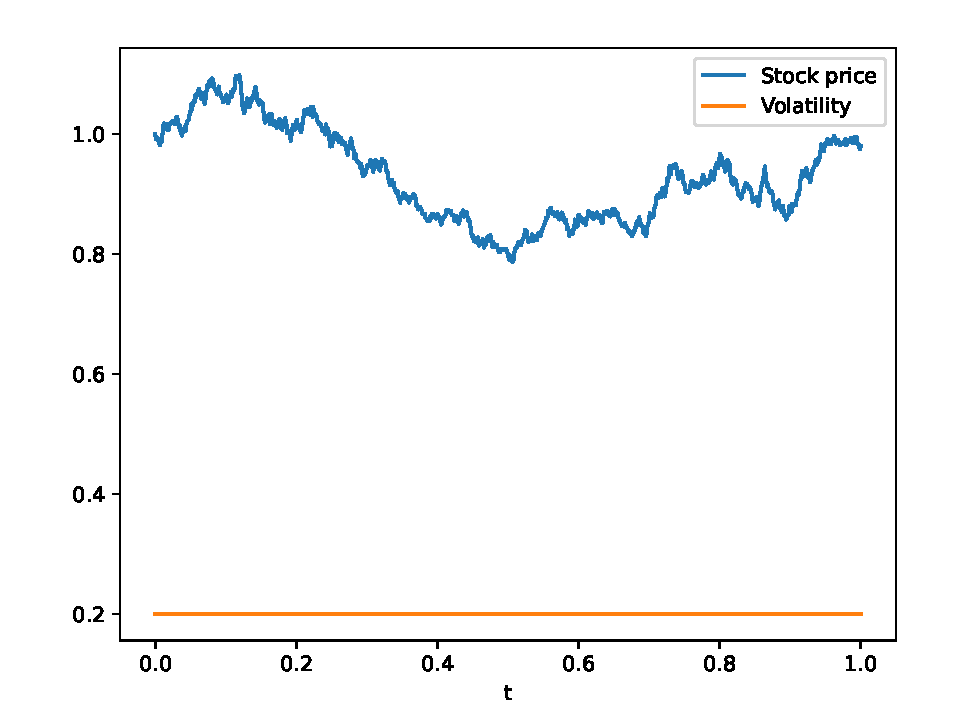
\includegraphics[width=1.05\linewidth]{BS_path.pdf}
  \caption{Black-Scholes}
\end{minipage}%
\begin{minipage}{.5\textwidth}
  \centering
  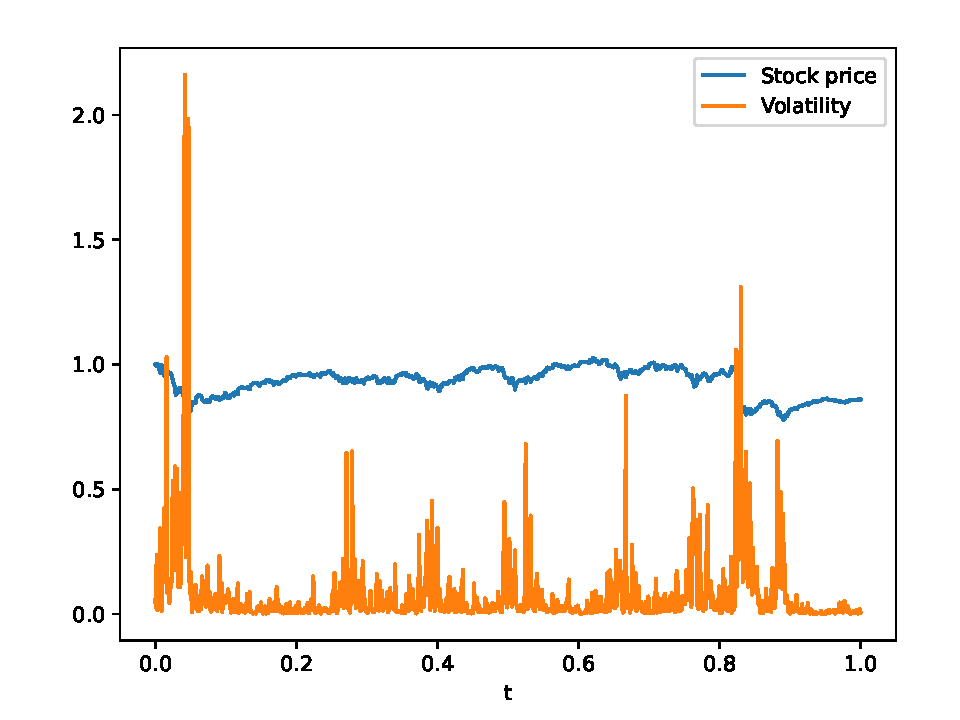
\includegraphics[width=1.05\linewidth]{rBergomi_path.pdf}
  \caption{Rough Bergomi}
\end{minipage}
\end{figure}


\end{frame}

\begin{frame}{Stochastic Volterra equations}
\only<1->{Consider general stochastic Volterra equation

$$X_t = X_0 + \int_0^t K(t-s) b(X_s) ds + \int_0^t K(t-s) \sigma(X_s) dW_s,$$

where $b,\sigma$ are Lipschitz and $K(t) = t^{H-1/2}$.}

\only<2->{Note that $$K(t) = c_H \int_0^\infty e^{-xt} x^{-H-1/2} dx.$$}

\only<3->{Idea: Approximate $K$ by $$\widehat{K}(t) = \sum_{i=1}^N w_i e^{-x_it}$$ and solve $$\widehat{X}_t = X_0 + \int_0^t \widehat{K}(t-s) b(\widehat{X}_s) ds + \int_0^t \widehat{K}(t-s) \sigma(\widehat{X}_s) dW_s.$$}
\end{frame}

\begin{frame}{Markovian structure}
\only<1->{\begin{proposition}[Abi Jaber, El Euch, 2019; Alfonsi, Kebaier, 2021]
The process $\widehat{X}$ is the solution to an $N$-dimensional ordinary SDE.
\end{proposition}}

\vspace{30pt}

\only<2->{\begin{theorem}[Alfonsi, Kebaier, 2021]
There exists a constant $C$ depending only on $H$, $b$, $\sigma$ and $T$, such that $$\E|X_T - \widehat{X}_T|^2 \le C\int_0^T |K(t) - \widehat{K}(t)|^2 dt.$$
\end{theorem}}

\vspace{30pt}

\only<3->{Question: How to choose nodes $(x_i)$ and weights $(w_i)$?}
\end{frame}

\begin{frame}{Previously known convergence rates}
\only<1->{\begin{theorem}[Alfonsi, Kebaier, 2021]
Truncate the domain of integration to $[0,L]$ and partition $[0,L]$ into $N$ equisized intervals. Use midpoint rule on these intervals. Then, $$\E|X_T - \widehat{X}_T|^2 \le C N^{-2H/3}.$$

Using more sophisticated point set of similar structure, we have almost rate $N^{-H}$.
\end{theorem}}

\vspace{30pt}

\only<2->{\begin{theorem}[Harms, 2019]
Special case of fractional Brownian motion (i.e. $b\equiv 0$, $\sigma\equiv 1$): Truncate domain of integration to $[\xi_0, \xi_n]$ and partition $[\xi_0,\xi_n]$ into $n$ geometrically spaced intervals. Use Gaussian quadrature of level $m$ on each of these intervals. Then, $$\E|X_T - \widehat{X}_T|^2 \le C(m) n^{-2Hm/3}.$$
\end{theorem}}
\end{frame}

\begin{frame}{Improved point set}
\only<1->{\begin{theorem}[Bayer, B., 2021]
Truncate the domain of integration to $[\xi_0,\xi_n]$ and partition $[\xi_0,\xi_n]$ into $n$ gemetrically spaced intervals. Use Gaussian quadrature of level $m$ on each of these intervals. Add an additional node at $x_0 = 0$. For the correct (known) choice of $m$, $\xi_0$ and $\xi_n$, we have, with $N=nm$, $$\E|X_T - \widehat{X}_T|^2 \le C N^{0.21}\exp\bigg(-\frac{2.1283}{A_H}\sqrt{N}\bigg),$$ where $$A_H = \bigg(\frac{1}{H} + \frac{1}{3/2-H}\bigg)^{1/2}.$$
\end{theorem}}

\only<2->{Numerical experiments suggest that we can even get $$\E|X_T - \widehat{X}_T|^2 \le C \exp\bigg(-\frac{3.6}{A_H}\sqrt{N}\bigg)$$ using a smarter choice of $m$, $\xi_0$ and $\xi_n$.}
\end{frame}

\begin{frame}{Numerics for fractional Brownian motion with $H=0.1$}
\begin{figure}
\centering
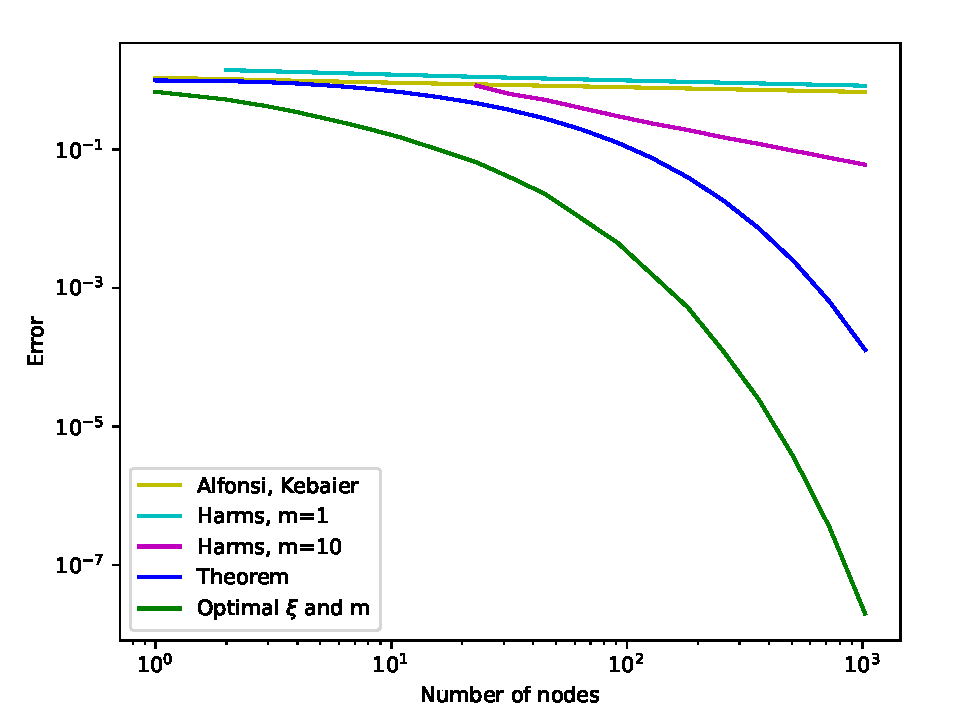
\includegraphics[scale=1.2]{fBm.pdf}
\end{figure}
\end{frame}

\begin{frame}{Rough Bergomi implied volatility smile with $H=0.07$}
\begin{figure}
\centering
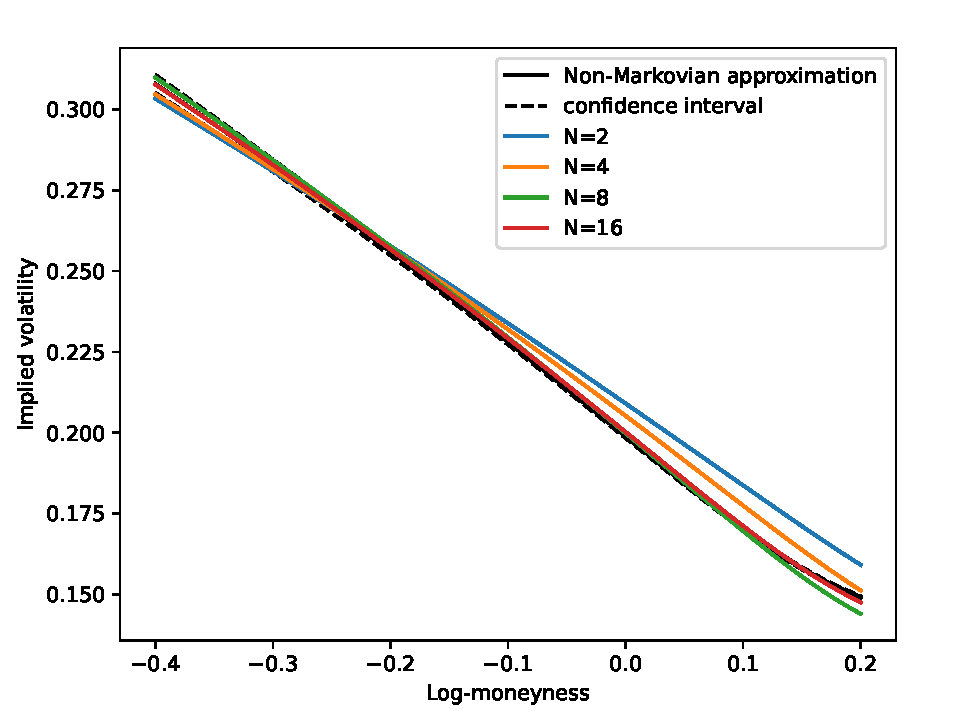
\includegraphics[scale=1.2]{rBergomi.pdf}
\end{figure}
\end{frame}

\begin{frame}{Rough Bergomi implied volatility smile with $H=0.07$}
\begin{figure}
\centering
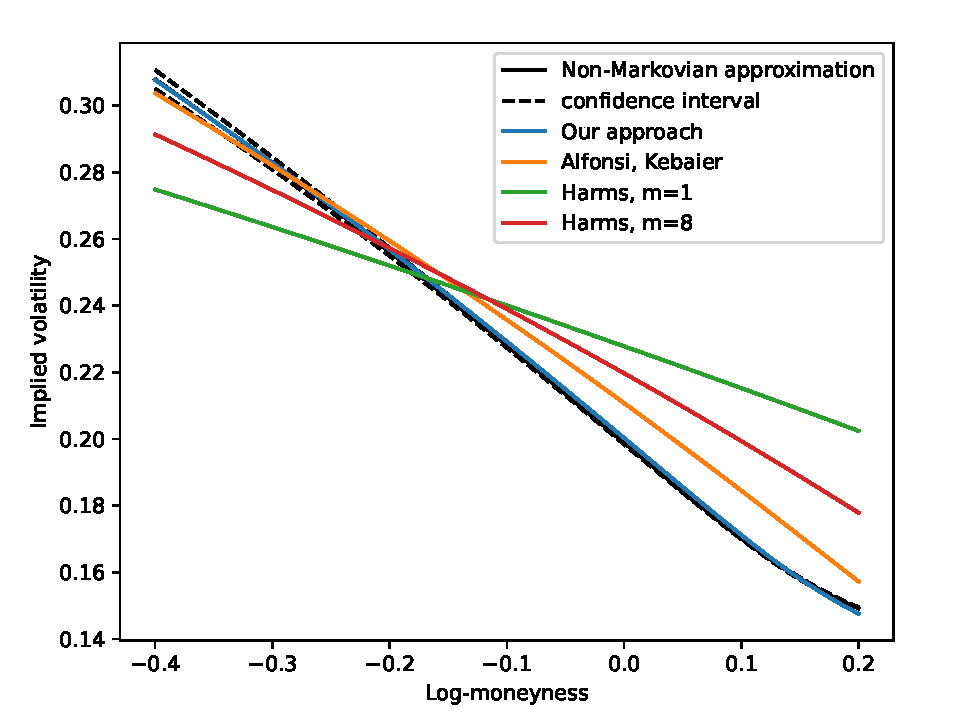
\includegraphics[scale=1.2]{rBergomi_comparison.pdf}
\end{figure}
\end{frame}

\begin{frame}{Rough Heston implied volatility smile with $H=0.1$}
\begin{figure}
\centering
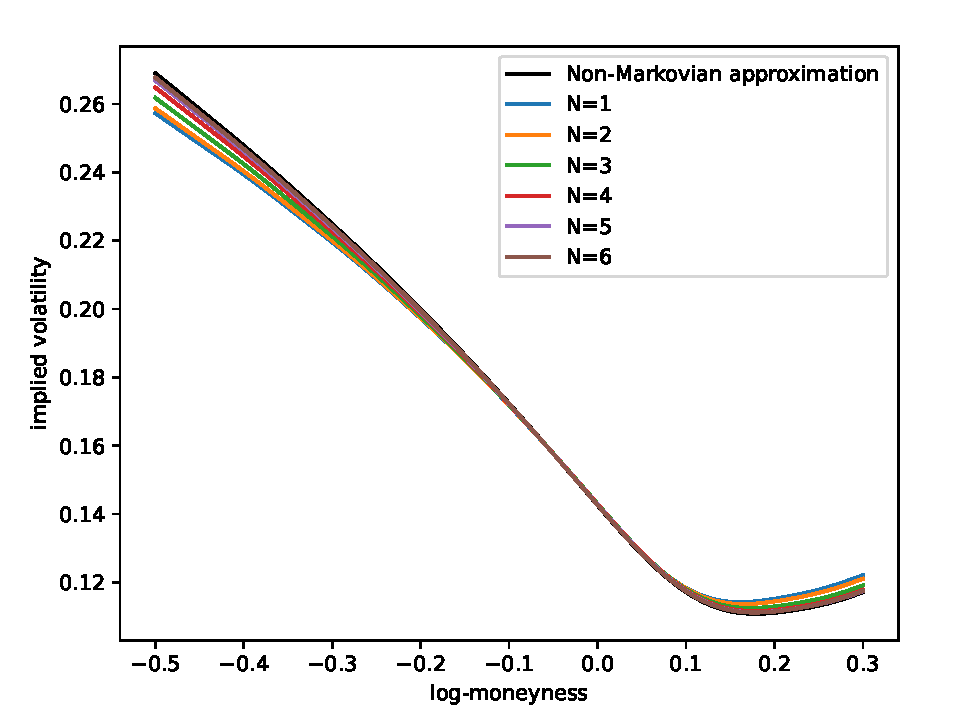
\includegraphics[scale=1.2]{rHeston.pdf}
\end{figure}
\end{frame}

\begin{frame}{Rough Heston implied volatility smile with $H=0.1$}
\begin{figure}
\centering
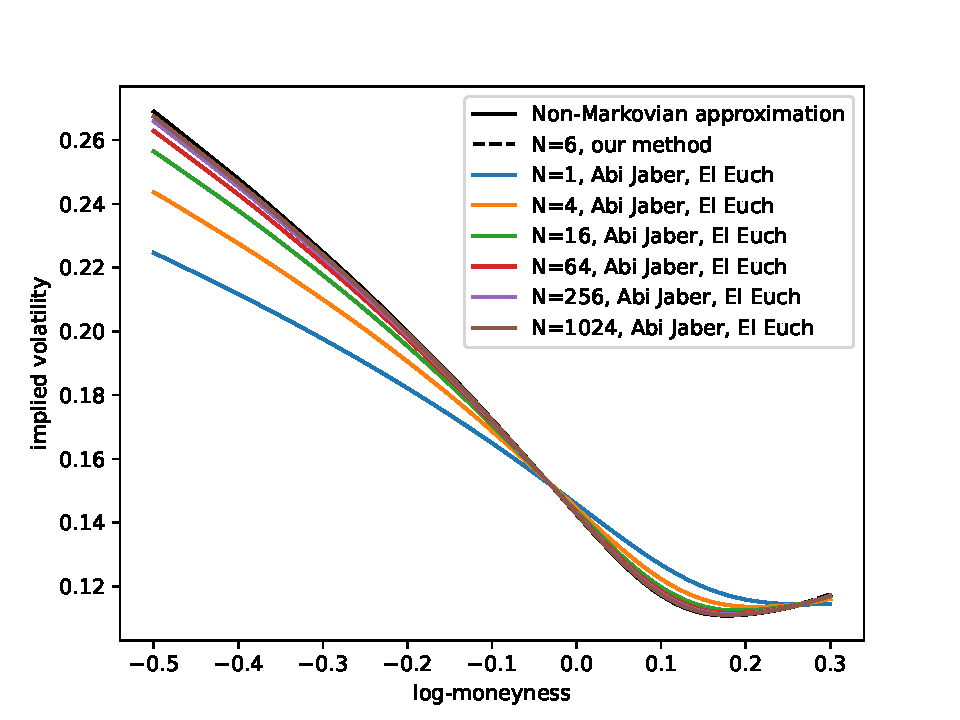
\includegraphics[scale=1.2]{rHeston_comparison.pdf}
\end{figure}
\end{frame}

\begin{frame}
\vspace{180pt}
\fontsize{48}{48}\selectfont
\begin{center}
Thank you for your attention!
\end{center}
\end{frame}

\end{document}
